%%%%%%%%%%%%%%%%%%%%%%%%%%%%%%%%%%%%%%%%%%%%%%%%%%%%%%%%%%%%%%%%%%%%%%%%%%%%%%%%
%2345678901234567890123456789012345678901234567890123456789012345678901234567890
%        1         2         3         4         5         6         7         8

\documentclass[letterpaper, 10 pt, conference]{ieeeconf}  % Comment this line out if you need a4paper

%\documentclass[a4paper, 10pt, conference]{ieeeconf}      % Use this line for a4 paper

\IEEEoverridecommandlockouts                              % This command is only needed if 
                                                          % you want to use the \thanks command

\overrideIEEEmargins                                      % Needed to meet printer requirements.

%In case you encounter the following error:
%Error 1010 The PDF file may be corrupt (unable to open PDF file) OR
%Error 1000 An error occurred while parsing a contents stream. Unable to analyze the PDF file.
%This is a known problem with pdfLaTeX conversion filter. The file cannot be opened with acrobat reader
%Please use one of the alternatives below to circumvent this error by uncommenting one or the other
%\pdfobjcompresslevel=0
%\pdfminorversion=4

% See the \addtolength command later in the file to balance the column lengths
% on the last page of the document

% The following packages can be found on http:\\www.ctan.org
%\usepackage{graphics} % for pdf, bitmapped graphics files
%\usepackage{epsfig} % for postscript graphics files
%\usepackage{mathptmx} % assumes new font selection scheme installed
%\usepackage{times} % assumes new font selection scheme installed
%\usepackage{amsmath} % assumes amsmath package installed
%\usepackage{amssymb}  % assumes amsmath package installed
\usepackage{algorithm}
\usepackage{algorithmic}
\usepackage{indentfirst}
\usepackage{amsmath}
\usepackage{graphicx}
\usepackage{stfloats}
\title{\LARGE \bf
A Sequence-Based Visual Place Recognition Technique with Segmented Database and Compact Sequence List
}


\author{Xin-Zhuo Li$^{1}$, Ning Ding$^{2}$ and Hung-Chyun Chou$^{3}$% <-this % stops a space
\thanks{*This work was supported in part by�National Key R\&D Program of China (2019YFB1310403, 2019YFB1310402), NSFC (U1813216, U2013202), and the Guangdong Basic and Applied Basic Research Foundation under Grant No. 2019A1515111119, 2021A1515010926, 2021B1515420005. *Corresponding author: Hung-Chyun Chou, Email: zhouhongjun@cuhk.edu.cn}% <-this % stops a space
\thanks{$^{1}$Xin-Zhuo Li is with Beijing Jiaotong University, Beijing, 100044, China.
		{\tt\small lixinzhuo323@outlook.com}}%
\thanks{$^{2}$Ning Ding is with Shenzhen Institute of Artificial Intelligence and Robotics for Society, and Institute of Robotics and Intelligent Manufacturing,The Chinese University of Hong Kong, Shenzhen, Shenzhen, Guangdong, 518172, China.�
	{\tt\small dingning@cuhk.edu.cn}}%
\thanks{$^{3}$Hung-Chyun Chou is with Shenzhen Institute of Artificial Intelligence and Robotics for Society, and Institute of Robotics and Intelligent Manufacturing,The Chinese University of Hong Kong, Shenzhen, Shenzhen, Guangdong, 518172, China.�
        {\tt\small zhouhongjun@cuhk.edu.cn}}%
}


\begin{document}



\maketitle
\thispagestyle{empty}
\pagestyle{empty}


%%%%%%%%%%%%%%%%%%%%%%%%%%%%%%%%%%%%%%%%%%%%%%%%%%%%%%%%%%%%%%%%%%%%%%%%%%%%%%%%
\begin{abstract}
	
Sequence-based visual place recognition algorithms have been proved to be able to handle environmental changes caused by illumination, weather, and time of the day with hand-crafted descriptors. However, exhaustive search for all images in query sequence is computationally expensive. In this paper, we propose a technique that can significantly reduce the size of searching space for sequence match while remaining a state-of-the-art accuracy. Firstly, we managed to achieve a better selection for reference candidates of images in query sequence by segmenting database according to similarity. Then, a much more informative and compact query sequence is designed by removing all the unnecessary images in origin query sequence. State-of-the-art performance is reported on public dataset with challenging environmental changes. Our algorithm shows comparable accuracy with other current best results, and exceeds all the other methods in the dataset with illumination variation. In addition, the decrease of execution time and higher success rate for selecting candidates of query images for sequence match are also provided.   

\end{abstract}


%%%%%%%%%%%%%%%%%%%%%%%%%%%%%%%%%%%%%%%%%%%%%%%%%%%%%%%%%%%%%%%%%%%%%%%%%%%%%%%%
\section{INTRODUCTION}

Visual place recognition (VPR) as a sub-domain of simultaneous localization and mapping (SLAM) has been widely discussed in recent years because of its contribution to the loop closure step in SLAM system. Recognizing a previously visited place correctly is indispensable for the subsequent optimization. In general, VPR can be considered as an image retrieval problem of finding the most similar matches of the query single-frame or sequence of frames in the reference database built by previous traverse. However, viewpoint variation, varied illumination and weather conditions could lead to different appearance of the same place which increase the difficulty of the recognition task significantly. Currently, CNN-based VPR techniques have succeeded on the most challenging VPR datasets, as evaluated in [1] and [2]. However, in order to train a CNN for VPR tasks, large-scale datasets from different environments under various angles, seasons and illumination conditions are needed. Moreover, the CNN's encoding-time and run-time memory are much higher than those required for the handcrafted descriptors. Although the CNN-based VPR techniques have outperformed handcrafted descriptor-based techniques currently, their intense computational requirement is still a serious problem.

Instead of using CNN-based VPR algorithms, sequence-based method has also demonstrated impressive performance in recognizing places that underwent severe appearance changes with handcrafted descriptors. In SeqSLAM [3], much better performance has been shown comparing to previous single-frame SLAM algorithms like FAB-MAP 2.0 [4]. However, exhaustive sequence search is computationally costly in large database. The sequence match procedure basically contained two steps. First step is evaluating all the reference images in database to generate a distance vector for every query frame in sequence and combining all the distance vectors to get a holistic distance matrix. And the second step is finding the best matching sequence in that distance matrix. In order to reduce the computational time in first step, retrieval techniques based on data structures like trees [5][6], graphs [7][8][9] and hashing [10][11][12] has been used in previous researches. As for the second step, we can either select a limited number of reference candidates for each query frame in sequence or set dynamic length of the sequence to reduce the size of the distance matrix. Our method integrates techniques of both steps together and use the information generated from first step to achieve a better performance in second step with no extra computation.

In this paper, we propose a novel VPR solution by utilizing the similarity of images to segment database and simplify query sequence. Firstly, a hierarchical retrieval in segmented database for each frame in query sequence is implemented to reduce single-frame searching time. As for sequence match, candidates of each query image will be selected to avoid exhaustive search in whole database. The segmentation of database also helps to exclude clustering incorrect reference images in candidates selection. Unnecessary interval images which can provide little supplementary information in a sequence are also ignored to achieve a more compact query list. After all the manipulation, the searching space for sequence match can be reduced significantly to achieve computational efficiency. Additionally, most of previous sequence-based algorithms assume a constant velocity between consecutive samples of reference and query data, which makes them unreliable in practice when velocity changed or robot kidnapping occurred. In our algorithm, such assumption is not needed. Instead, we use the similarity between images to ensure the same distance of adjacent query frames in sequence and their corresponding reference images. In other words, the constraint we use to find sequence in database is from similarity calculation instead of invariant velocity assumption. In general, the main contributions in this paper will be listed below:

\begin{itemize}
	\item Use similarity between images to segment database to achieve a hierarchical searching method
	\item Better performance of candidates selection for query frames in sequence with the help of database segmentation
	\item Significantly simplify sequence match by removing all the unnecessary interval images in query sequence to achieve a much more compact query list
	\item Utilize the same similarity threshold for both database and query images to avoid using searching method based on invariant velocity assumption.
	
\end{itemize}

The rest of the paper is organized as follows. In Section II, we summarize relevant prior research in VPR. Section III describes our algorithm, both the single-frame retrieval and sequence match method will be illustrated.  Our experimental design and results are presented in Section IV, focusing on the accuracy of our algorithm and the reduction of execution time.

\begin{figure*}[t]
	\centering
	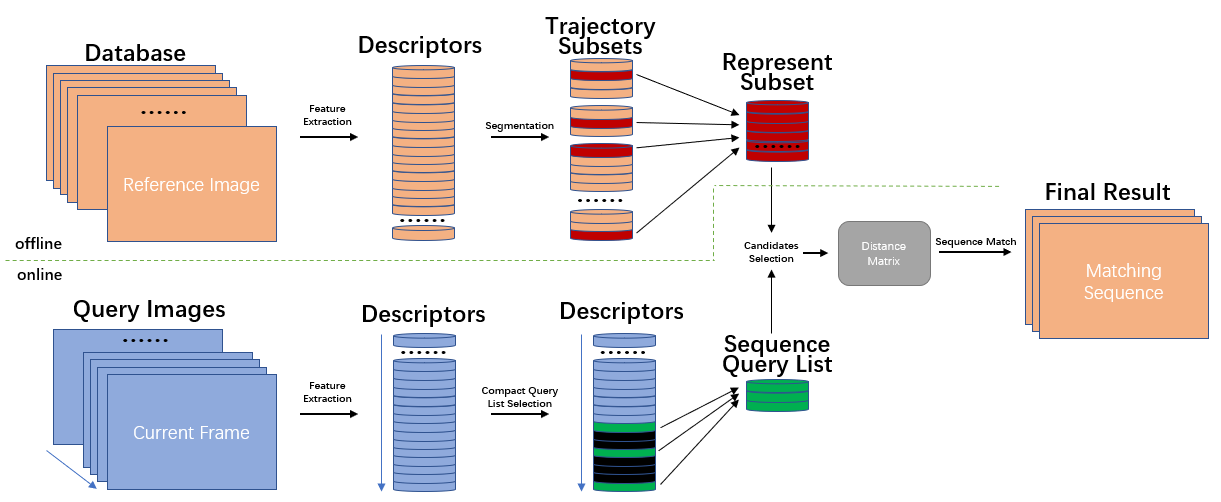
\includegraphics[scale=0.65]{fig_1.png}
	\caption{The general procedure of our sequence-based VPR technique}
	\label{figurelabel}
\end{figure*}
\section{RELATED WORK}
After SeqSLAM [3] was proposed, many following researches have been done to solve the high computational cost problem. For example, Fast-SeqSLAM [13] used an approximate nearest neighbor algorithm [14] to search for $u$ nearest neighbor images for a current view where $u$ is constant and much smaller than the number of images in the database. Then, a sparse matrix is created for subsequent sequence match. For each frame in the query list, only few candidates is remained in this matrix. As in DOSeqslam [15], the incoming image stream is segmented to using loop closure detection techniques to decrease the searching domain in the database. In their method, whether two images share a common local descriptor is used to evaluate similarity between images, which lead to a dynamic sequence length. While in ConvSequential-SLAM [16], the author proposed a concept of information gain to evaluate whether the sequence length is enough for matching. They utilized Histogram-of-Oriented-Gradients (HOG) descriptors and entropy map representing the salient regions in each query image to compute the information gain. New frames will be added to the sequence successively until the sequence reaches required information gain. This also helped them to achieve a dynamic sequence length. 

Even though all these algorithms managed to be more computationally efficient comparing to SeqSLAM by reducing the size of searching space, they are still based on the invariant velocity assumption. Moreover, similar adjacent images in query sequence which can provide little supplementary information for retrieval were being exhaustively matched in their methods. Although dynamic sequence length has been used in previous research because the performance of sequence match is strongly related to sequence length, the fact that similar query images in a sequence are abundant has not been realized yet.


\section{METHODOLOGY}
This section presents the methodology proposed in our work, including modified information gain computation method, segmentation of database, hierarchical retrieval strategy based on segmentation, simplification of query sequence and how to implement sequence match with previously generated features. The general procedure is shown in Fig. 1. For the offline processes, the descriptors of reference images in database will firstly be calculated. Secondly, the database will be segmented by putting similar adjacent images in one subset. Each subset represents a trajectory of the traverse. Then the most informative image in each trajectory subset which can represent all images in this set will be gathered into the represent subset whose size is much smaller than the database. For the online processes, the descriptors of query images will firstly be extracted as well. After that, the query sequence for the current frame is created by adding images before it with enough different features iteratively to obtain a list of size $M$. Only the green images in the graph will be added to the sequence, the black images are ignored because they are too similar to the current frame which can provide little additional information for the holistic sequence. Then, each query image will search their best match in represent subset to find best $N$ images. Further search in $N$ trajectory subsets that is represented by these best $N$ images will be carried out. Each trajectory subset will generate a local best match. These local best matches are gathered as candidates for query images. A distance matrix $D$ of size $M \times N$ that contains the similarity score between reference and query images is created subsequently. After sequence match in the space $D$, we can obtain the final matching sequence. Detailed information is provided by following subsections.

\subsection{Similarity and information gain}
In order to obtain the similarity between images, we applied a compute-efficient and training-free approach called CoHoG [17]. Firstly, query images are converted to grayscale and resized to $W1 \times H1$. Then, the entropy map of size $W1 \times H1$ of these images are used to extract regions-of-interest (ROI). A region in an image is defined as a $W2 \times H2$ image patch. Thus, these $W1 \times H1$ images with regions/patches of size $W2 \times H2$ each contains $RN$ regions, where $RN = (H1/H2)\times(W1/W2)$. The goodness matrix $R$ based on the entropy map as shown below is then generated. Element $r_{ij}$ in $R$ equals to 1 when entropy score $e_{ij}$ is greater than or equal to the goodness threshold $GT$, which means this region will be selected for matching. Only $G$ regions which is informative enough for matching will be remained after this step. 

\begin{equation}
\boldsymbol{R}=
\begin{bmatrix}
r_{11} & r_{12}  & \cdots   & r_{1j}   \\
r_{21} & r_{22}  & \cdots   & r_{2j}  \\
\vdots & \vdots  & \ddots   & \vdots  \\
r_{i1} & r_{i2}  & \cdots\  & r_{ij}  \\
\end{bmatrix}
\end{equation}
\begin{center}
if $e_{ij} >= GT$, $r_{ij} = 1$;  else, $r_{ij} = 0$ \\
\end{center}
A corresponding HOG-descriptor of depth $4\times L$ will be calculated for each ROI next. The query image HOG-descriptor is now a two-dimensional matrix with dimensions $[G, 4 \times L]$. After that, standard matrix multiplication between query and reference descriptor matrix and max pooling for the generated matrix will be implemented. In the end, we can get the similarity score in the range of 0 to 1. 

Then, the similarity of images can be used to generate the information gain. The feature information gain is defined in [16] to determine if the information contained by a sequence is enough after adding a new frame to the sequence. By keeping comparing the similarity score between first and subsequent images with the threshold to determine if newly added frame have provided sufficient information gain. However, in this research, the threshold to determine whether two images are similar enough is the same for all the images. In other words, when the similarity score between first image and newly added image is smaller than a same constant number, they assumed enough information gain have been achieved. In fact, when a same group of images is comparing to two different images, their averages of similarity score will be different, which means a constant threshold can't guarantee the same information gain for all images. So, they also had to set a limit for the number of added comparing images before obtaining enough information gain when the threshold is not appropriate. To solve this problem, we initialize a subset with two adjacent images $ref_1$, $ref_2$ to get a suitable threshold for each subset. The similarity score of these two images will be stored as $S_{init}$ which is generally the highest score because of the sequential nature of database. Then, similarity score between  $ref_1$ and following images $ref_3,ref_4 \cdots$ will be compared to $S_{init}$ minus a Difference Threshold $DT$ to determine the information gain. In addition, we also discovered a trend that as the image comparison continued the similarity score between initial image and current comparing image will descend obviously, but when the score suddenly rises comparing to last score, this implies that the current image has contained enough new descriptors which can randomly generate higher scores. In this case, we also consider enough information gain has been achieved.  So, two new constraints which is now our new information threshold to evaluate information gain are shown below. If any of them has been satisfied, the sequence reaches sufficient information gain.

\begin{equation} 
\left\{
\begin{aligned}
\begin{array}{lr}
S<S_{init} - DT\\ 
S>S_{last}\\ 
\end{array}
\end{aligned} 
\right. 
\end{equation}
 
\subsection{Segmentation of reference database}
 
Similarity score between one query image and two similar (usually adjacent in database) reference images tend to be close. Therefore, if a set of images is similar enough, we can choose one image to represent the whole set. In this way, we can simplify the entire database into a set of represent images to achieve hierarchical retrieval like [10]. However, in our method the clustering procedure is not conducted through the database for all images. Instead, temporal consistence inside each subset is required. We divide the database subsequently from the first reference frame using information gain to generate sequence subsets. The selection of represent image for each subset is determined by the number of regions in each image from ROI extraction, which is mentioned in Section III-A. The image with most regions is considered to be most informative and can better describe its whole set. Then, all these represent images in each subset are combined to form a represent set. The represent set's size is much smaller than the origin database. Each element in this set leads to a subset with similar frames. A two-dimensional set that stores every frame's descriptors is also created accordingly. The algorithm of whole segmentation process can be found in Algorithm 1.
 
The reason why segmenting database subsequently in temporal order instead of clustering most similar images through the whole database is because two adjacent reference images tend to have similar scores even if they are both wrong. Instead of blindly relying on scores, which can lead to all candidates falling into an incorrect location with many high score frames, our segmentation strategy provides more options of different locations in candidates selection. 

\begin{algorithm}[t]
	\caption{Segment database} 
	\label{alg3} 
	\begin{algorithmic}
		\REQUIRE  ~~\\
		The reference database, $DB$ \\
		$n^{th}$  images in $DB$, $ref_n$ \\ 
		\ENSURE A two-dimensional set containing all the segmented subsets, $subset$ 
		\STATE $m = 0$
		\STATE $n = 0$
		\WHILE{$n < length(DB)$} 
		\STATE $flag = 0$
		\STATE $last\_score = 1 $
		\STATE $subset[m][0]= ref_{n}$ 
		\STATE $subset[m][1]= ref_{n+1}$ 
		\STATE $init\_score = similarity\_compute\_func(ref_{n},$\\
		$ref_{n+1})$ 
		\STATE $k = 2$
		\WHILE{$flag = 0$}
		\STATE $curr\_score = similarity\_compute\_func(ref_{n},$\\
		$ref_{n+k})$ 
		\IF {$curr\_score < init\_score - DT$ \textbf{or} $curr\_score > last\_score$}
		\STATE $flag = 1$ 
		\STATE $n = n + k $ 
		\STATE $m = m + 1 $ 
		\ELSE 
		\STATE $subset[m][k]= ref_{n+k}$ 
		\STATE $k= k + 1$ 
		\STATE $last\_score = curr\_score$ 
		\ENDIF
		\ENDWHILE  
		\ENDWHILE 
		\RETURN $subset$  
	\end{algorithmic} 
\end{algorithm}

\subsection{Hierarchical retrieval}
The process of the single-frame retrieval is illustrated in this section. Firstly, the similarity score between the query image and all the images in the represent set will be calculated. The HoG descriptor computation and ROI extraction will be implemented for query image, and descriptors for reference image has been stored previously. Then, only frames with top-$N$ scores will be remained. After that, all similarity scores between query image and images in $N$ subsets which are represented by the $N$ represent images will be computed. Every subset will generate a local best matching image. The image with the highest score in $N$ images is considered to be the final best match in single-frame retrieval scenario. As for sequence match, all the best $N$ images and their indexes in database will be stored for following steps. 
 
\subsection{Sequence query list generation}
Sequence-based VPR algorithm is more robust comparing to single-frame method because of supplementary information is provided by frames before current frame. Generally, the longer sequence contains more information and results in better performance. However, information gain is the actual feature that strongly influences the performance, instead of sequence length. More exactly, the enhancing effect of a newly added frame in sequence is determined by its dissimilarity with the current frame. In other words, including two similar images in a sequence can not improve the retrieval performance comparing to include only one of them. The procedure to create our sequence query list is similar to ConvSequential-SLAM [16], keep comparing new frames before current frame until the sequence information gain reaches the threshold. But, only the frame at where the threshold is just reached  will be added to the sequence list, and all the interval images between this image and current image will be ignored. After a new frame is added to the sequence list, the newly added frame will now be regarded as current frame to find the next frame being added to the list.  In our method, new images will be added to the sequence list iteratively $M-1$ times to create a sequence list of size $M$.


\begin{figure*}[b]
	\centering
	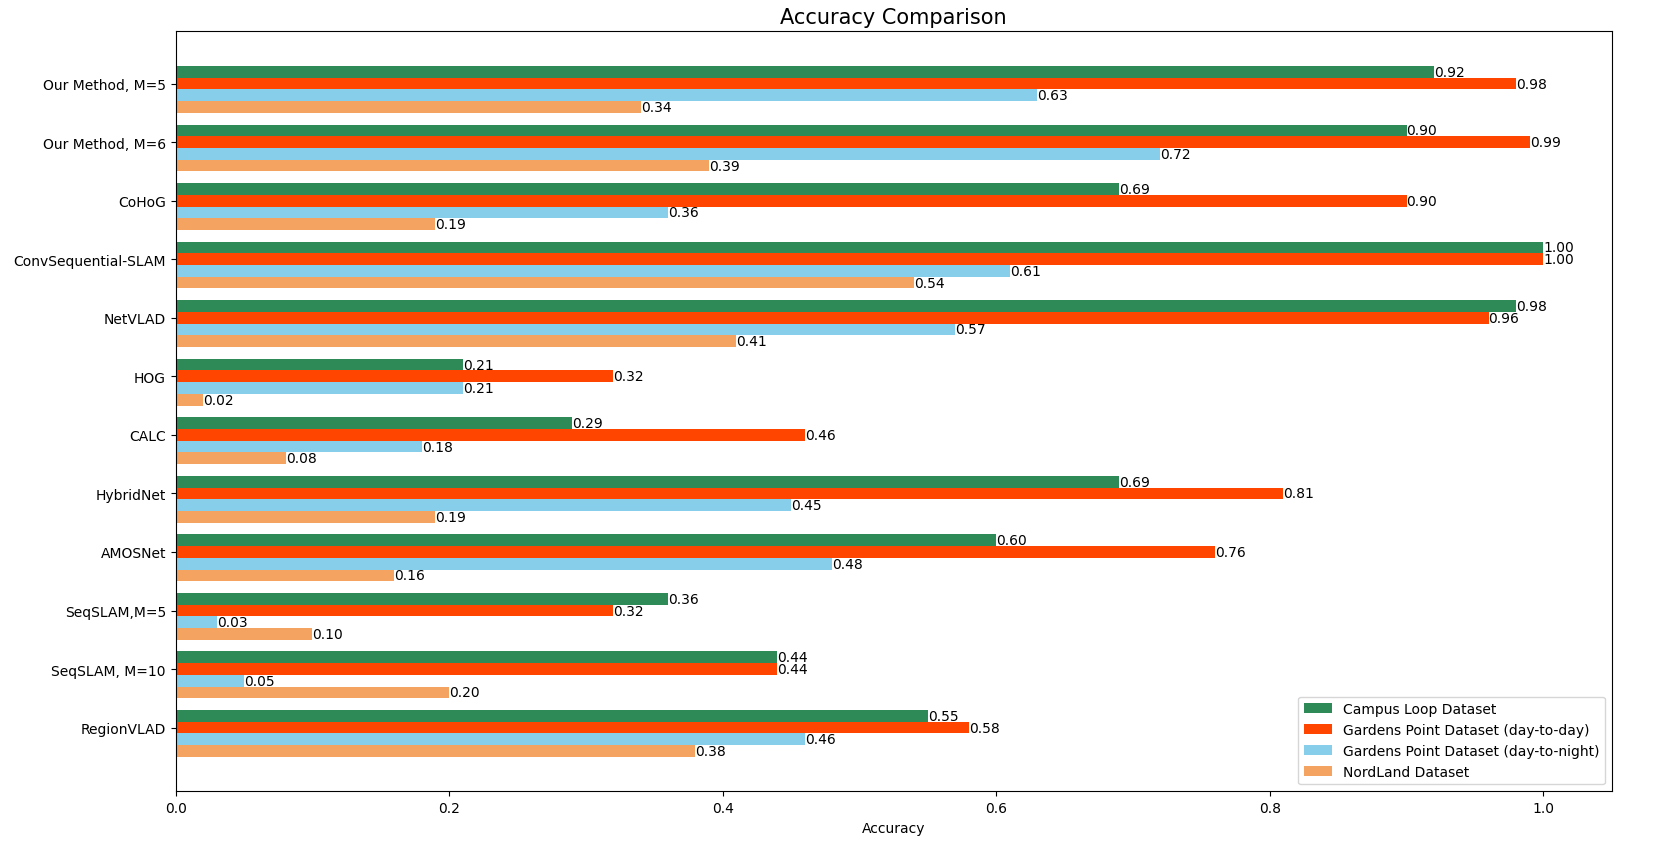
\includegraphics[scale=0.31]{fig_2.png}
	\caption{Accuracy Comparison with other VPR algorithms}
	\label{figurelabel}
\end{figure*} 
\subsection{Sequence match}


After all the manipulations mentioned above, we obtain a distance matrix $D$ of size $M \times N$, where $M$ is the length of the query list and $N$ is the number of candidate reference images for each element in that list. The matrix $D$ as shown below contains $M \times N$ similarity scores between query and reference images. Since the sequence retrieval is limited in this constant size matrix, we can achieve a $O(1)$ complexity in this sequence matching procedure. In addition, the indices of reference frames in the database is also stored for later filtering process. 
\begin{equation}
\boldsymbol{D}=
\begin{bmatrix}
d_{11} & d_{12}  & \cdots   & d_{1n}   \\
d_{21} & d_{22}  & \cdots   & d_{2n}  \\
\vdots & \vdots  & \ddots   & \vdots  \\
d_{m1} & d_{m2}  & \cdots\  & d_{mn}  \\
\end{bmatrix}
\end{equation}
\begin{center}
     Where, $d_{ij}$ = similarity score between $i^{th}$ query image in sequence and $j^{th}$ candidate reference image \\
\end{center}

Most of previous sequence-based VPR algorithms evaluate sequence score based on trajectory velocity, which is varied between $V_{min}$ and $V_{max}$ in steps of $V_{step}$. The sequences of different velocities in the map will be evaluated to find the best match. This sequence matching strategy assumed that the velocity during query and reference sequence is constant, which makes it unreliable in reality. The constant velocity brings fixed frame indices interval between consecutive images in sequences which is an extremely useful constraint to find sequences of images in searching space. While in our method indices interval between images is based on information gain, and the same distance between consecutive images is not needed. So, such assumption is avoided in our method. Instead, we use three constraints as shown below to generate a trajectory in the searching space for evaluation. 
\begin{equation} 
\left\{
\begin{aligned}
\begin{array}{lr}
R_1<R_2<\cdots<R_m \\ 
R_k>RL_{k+1}|k\in[1,m-1]\\ 
\mathop{\arg\max}\limits_{\boldsymbol{score}} \sum\limits_{k=1}\limits^{m}{score_k}\\
\end{array}
\end{aligned} 
\right. 
\end{equation}

Where $R_k$ is the index of corresponding reference image in database for $k^{th}$ query image in sequence list. The first inequality requires query and reference images must follow the same temporal order. Because the frame indices interval between adjacent images in the query list and their matching reference images should be close. We define the distance between one image in sequence list and the image that is added after it into query sequence is one $IT$, because new image is added when sequence reaches the information threshold exactly once. Applying the same information threshold as creating query sequence list to all reference images in database twice, we can get the image that is two $IT$ before every reference image. These images are gathered into the $RL$ set. And $RL_k$ is the index of corresponding image in $RL$ for $k^{th}$ query image in sequence. Since the distance between two adjacent query images in sequence is one $IT$, their corresponding reference images should remain an approximate same distance as well. Therefore, the distance between two reference images must not exceed two $IT$, and this requires $R_k$ to be larger than $RL_{k+1}$. $score_1,score_2,\cdots, score_m$ represent the similarity score between each query frame and their candidates. After two filtering steps mentioned above, the combination of query images with highest summed score will finally be selected as the best match sequence.
 
\section{EXPERIMENTAL RESULTS}
 
 
\subsection{Datasets}
To evaluate our proposed technique, the following public VPR datasets are used: Gardens Point dataset [18] containing images  with viewpoint variation. This dataset consists of a total of 600 images, divided into 200 reference images (day images) and 400 query images, equally divided into day and night images. In this paper, we used day left as reference images, while day right and night right are used as query images. Nordland dataset [19] containing drastic appearance changes in different seasons. We have used first 200 query images taken from the summer dataset and first 200 reference images taken from the winter dataset. Campus Loop dataset [20] containing viewpoint variation, seasonal variation and also the presence of statically-occluded frames. This dataset contains 100 query and 100 reference images.


\subsection{Parameters}
The parameters for descriptors extraction we used in this work are, $W1 = H1 = 512$, $W2 = H2 = 16$, $L = 8$ bins, $GT$ = 0.5. As for the sequence match parameters, we set $DT$ = 0.03, $M$ = 5 and $M$ = 6, $N$ = 20. These values can provide a good performance in all the datasets we tested. Especially, the values of $M$, $N$ could be set much smaller to obtain a faster online matching in a less challenging environment that didn't involve day-night or seasonal variation. For example, in the Gardens Point dataset (day-to-day), we set $M = 3, N= 5$ and still achieve an almost same accuracy as current $M$, $N$ values. The influence of $M$, $N$ on searching results will be well illustrated in Section IV-E and Section IV-F.

 

\subsection{Accuracy comparison}
In our experiment, we use Intersection over Union (IoU) of two sequences to determine if two sequences are close enough to represent a same location. When IoU equals 0, this means the trajectories of two sequences are totally irrelevant. And when IoU is larger than 0.5, this indicates the majority of two trajectories are overlapping at a common place. So in this case, we consider two trajectories are close enough and designate two sequences as a correct match. The IoU will be calculated according to frame indices in practical.

Then the accuracy of our algorithm has been compared with other previous research, such as ConvSequential-SLAM [16], , NetVLAD [21], CoHOG [17], HOG [22],CALC [20], HybridNet [23], AMOSNet [23], SeqSLAM [3] and RegionVLAD [24] on the datasets mentioned in Section IV-A. The result is shown in Fig. 2. The parameter $M$ in the graph is the sequence length. It can be seen that our method has achieved a comparable performance with other state-of-the-art algorithms like NetVLAD and ConvSequential-SLAM. Comparing to our baseline method CoHoG, the performance has been improved significantly with supplementary sequential information. And our method outperformed all the other illustrated algorithms in the Gardens Point Dataset (day-to-night) which involves illumination variation. In addition, the results of our method with two different sequence lengths are illustrated to show the significant improvement in illumination and season variant dataset like Gardens Point dataset (day-to-night) and Nordland dataset caused by adding just one new frame in query sequence.

\subsection{Recall@k evaluation} 
\begin{table}[h]
	\caption{Recall@k of CoHoG and our method}
	\label{table_1}
	\begin{center}
		\begin{tabular}{|c||c|c|c|c|c|}
			\hline
			& k=1 & k=3 & k=5 & k=10 & k=20\\
			\hline
			CoHoG & 0.31 & 0.42 & 0.50 & 0.57 & 0.70\\
			\hline
			Our Method & 0.29 & 0.42 & 0.52 & 0.59 & 0.81\\
			\hline
		\end{tabular}
	\end{center}
\end{table}
We have proposed a hierarchical single-frame searching algorithm to achieve a faster retrieval speed comparing to the baseline method CoHoG. The reduction of execution time will be illustrated in Section IV-F. Before that, it is necessary to prove that our method can remain the same accuracy performance. We will use recall@$k$ as our performance metric to evaluate two method in the illumination-variant Gardens Point dataset(day-to-night). Recall@$k$ is defined as the ratio of correctly retrieved queries within the top $k$ predictions to the total number of queries. Specifically, Recall@1 can represent the accuracy of single-frame retrieval. However, the performance when $k$ increases is more important in our experiment because it is related to the selection of candidates for frames in query sequence. As shown in Table 1, two methods can achieve almost identically performance in single-frame retrieval, and our method gradually exceeds CoHoG when $k$ increases. This is because the segmentation of database help us to filtering out some high-score incorrect images clustering at false positive places. 


\subsection{Various sequence length performance} 
\begin{figure}[h]
	\centering
	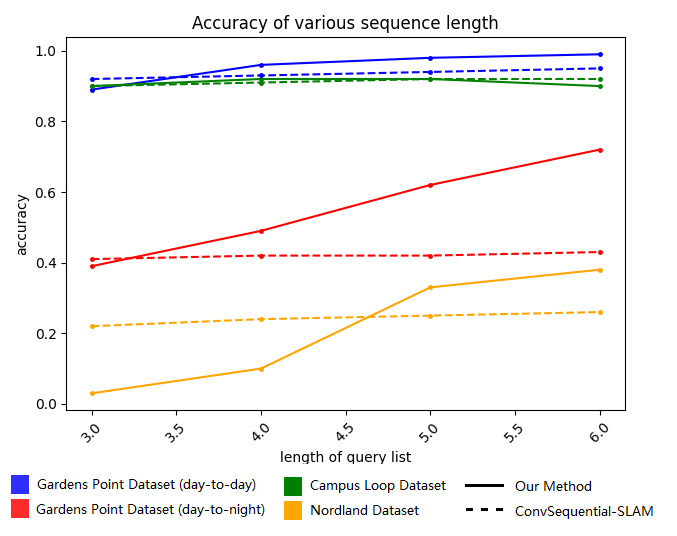
\includegraphics[scale=0.6]{fig_4.png}
	\caption{Performance comparison under different sequence length}
	\label{figurelabel}
\end{figure}
This section will show how the performance of our algorithm and ConvSequential-SLAM [16] varies because of changing sequence length. ConvSequential-SLAM is chosen because its descriptor extraction is also based on CoHoG, and it has managed to be one of the current state-of-the-art VPN algorithm. As shown in Fig. 3, the accuracy of two algorithms in Gardens Point dataset (day-to-day) and Campus Loop dataset which do not involve illumination variation is very close because the performance of single-frame retrieval for images in query sequence is already fairly good. So, we will mainly focus on the other two challenging datasets. According to the graph, the accuracy of ConvSequential-SLAM improved slightly with each new adding frame in sequence. However, each new frame can significantly boost our algorithm accuracy since the information gain provided by the new frame is much larger than previous sequence-based algorithm. Moreover, the performance of our method at length 5 is comparable to static ConvSequential-SLAM at length of 20. Hence, our algorithm has proved to achieve a much more informative and compact sequence list for sequence match.    

\subsection{Computational Efficiency}
\begin{figure}[h]
	\centering
	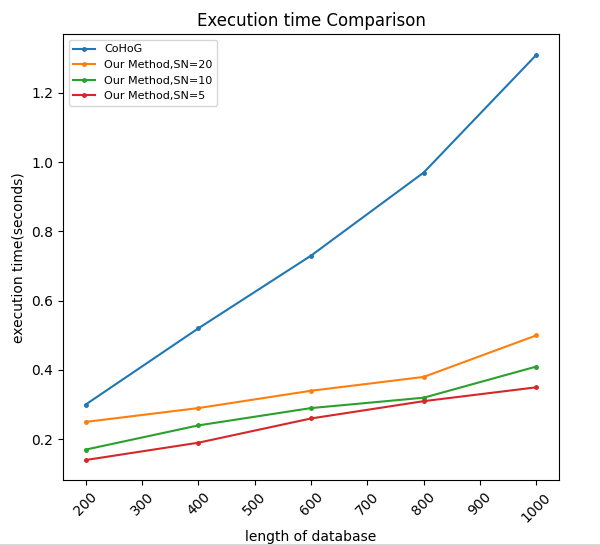
\includegraphics[scale=0.4]{fig_3.png}
	\caption{Execution time comparison with CoHoG}
	\label{figurelabel}
\end{figure}
The sequence-based VPR algorithms can be divided into two steps, single-frame candidates selection for query frame in sequence and evaluation of sequences composed of selected candidates. In the first step, we used a hierarchical searching method to avoid exhaustive search in whole database like our baseline algorithm CoHoG. Fig. 4 below shows the comparison of execution time between CoHoG and our algorithm with different $N$ values. Our method has much less execution time and smaller $N$ can further improve the performance.

In the second step, the sequence length of our method is much smaller than previous sequence-based VPR algorithms and can still achieve a state-of-the-art-performance. This is because our query sequence is much more compact and contains more information. Obviously, the computational time is strongly effected by the sequence length. Therefore, the reduction of sequence length lead to more computationally efficient VPR algorithm. Moreover, velocity searching which is very computationally expensive has been avoided during sequence match procedure. Instead, three constraints are applied, as showed in Section III-E to evaluate sequences in searching space. Two filters also helped to reduce the number of sequences needed to be evaluated in subsequent steps. Overall, benefitting from the strategies being applied in both steps, we managed to achieved a sequence-based algorithm with computational efficiency.  



%\section{CONCLUSIONS}
 

%\addtolength{\textheight}{-12cm}    
 


\begin{thebibliography}{99}
\bibitem{c1}M. Zaffar, A. Khaliq, S. Ehsan, M. Milford, and K. McDonald-Maier, "Levelling the playing field: A comprehensive comparison of visual place recognition approaches under changing conditions," 2019, arXiv:1903.09107. [Online]. Available: http://arxiv.org/abs/1903.09107
\bibitem{c2} M. Zaffar, A. Khaliq, S. Ehsan, M. Milford, K. Alexis, and K. McDonald-Maier, "Are state-of-the-art visual place recognition techniques any good for aerial robotics" 2019, arXiv:1904.07967. [Online]. Available: http://arxiv.org/abs/1904.07967
\bibitem{c3}M. J. Milford and G. F. Wyeth. "SeqSLAM: Visual route-based navigation for sunny summer days and stormy winter nights," In Proceedings of the IEEE International Conference on Robotics and Automation (ICRA), pages 1643-1649. IEEE, 2012.
\bibitem{c4}M. Cummins and P. Newman, "Highly scalable appearance-only SLAM - FAB-MAP 2.0," presented at Robotics: Science and Systems, Seattle, United States, 2009.
\bibitem{c5}Y. Hou, H. Zhang, and S. Zhou, "Tree-based indexing for real-time
convnet landmark-based visual place recognition," International Journal
of Advanced Robotic Systems, vol. 14, no. 1, p. 1729881416686951,
2017.
\bibitem{c6}D. Schlegel and G. Grisetti, "Hbst: A hamming distance embedding
binary search tree for feature-based visual place recognition," IEEE
Robotics and Automation Letters, vol. 3, no. 4, pp. 3741-3748, 2018.
\bibitem{c7}B. Harwood and T. Drummond, "Fanng: Fast approximate nearest
neighbour graphs," in Proceedings of the IEEE Conference on Computer
Vision and Pattern Recognition, 2016, pp. 5713-5722.
\bibitem{c8}M. G. Gollub, R. Dub�, H. Sommer, I. Gilitschenski, and R. Siegwart,
"A partitioned approach for efficient graph-based place recognition,"
in Proc. IEEE/RSJ Int. Conf. Intell. Robots Syst./Workshop Planning,
Perception Navigat. Intell. Veh., 2017.
\bibitem{c9}E. Garcia-Fidalgo and A. Ortiz, "Hierarchical place recognition for
topological mapping," IEEE Transactions on Robotics, vol. 33, no. 5,
pp. 1061-1074, 2017.
\bibitem{c10}S. Garg and M. Milford, "Fast, compact and highly scalable visual place recognition through sequence-based matching of overloaded representations," in Proc. IEEE Int. Conf. Robot. Autom. (ICRA), May 2020, pp. 3341-3348. 
\bibitem{c11}A. Andoni and P. Indyk, "Near-optimal hashing algorithms for
approximate nearest neighbor in high dimensions," in 2006 47th annual
IEEE symposium on foundations of computer science (FOCS-06).
IEEE, 2006, pp. 459-468.
\bibitem{c12}Y. Weiss, A. Torralba, and R. Fergus, "Spectral hashing," in Advances
in neural information processing systems, 2009, pp. 1753-1760.
\bibitem{c13}S. M. Siam and H. Zhang, "Fast-SeqSLAM: A Fast Appearance Based
Place Recognition Algorithm," in Proc. IEEE International Conference
on Robotics and Automation, 2017, pp. 5702-5708.
\bibitem{c14}P. Neubert, S. Schubert, and P. Protzel. "Exploiting intra database similarities for selection of place recognition candidates in changing environments," In Proc. of the CVPR Workshop on Visual Place Recognition in Changing Environments, 2015.
\bibitem{c15}Tsintotas, K.A.; Bampis, L.; Gasteratos, A. "DOSeqSLAM: Dynamic on-line sequence based loop closure detection algorithm for SLAM," In Proceedings of the 2018 IEEE International Conference on Imaging Systems and Techniques (IST), Krakow, Poland, 16-18 October 2018; pp. 1-6.f
\bibitem{c16} M.-A. Tomit -a, M. Zaffar, M. Milford, K. McDonald-Maier, and S. Ehsan, "Convsequential-slam: A sequence-based, training-less visual place recognition technique for changing environments," arXiv preprint arXiv:2009.13454, 2020
\bibitem{c17}M. Zaffar, S. Ehsan, M. Milford, and K. McDonald-Maier, "CoHOG: A light-weight, compute-efficient, and training-free visual place recognition technique for changing environments," IEEE Robot. Autom. Lett., vol. 5, no. 2, pp. 1835-1842, Apr. 2020.
\bibitem{c18}IEEE Robot. Autom. Lett., vol. 5, no. 2, pp. 1835-1842, Apr. 2020. N. Sunderhauf, S. Shirazi, F. Dayoub, B. Upcroft, and M. Milford, "On the performance of ConvNet features for place recognition," in Proc. IEEE/RSJ Int. Conf. Intell. Robots Syst. (IROS), Sep. 2015, pp. 4297-4304.
\bibitem{c19}S. Skrede. (2013). Nordland Dataset. [Online]. Available: https://nrkbeta.no/2013/01/15/nordlandsbanen-minute-by-minute-season-by-season/
\bibitem{c20}N. Merrill and G. Huang, "Lightweight unsupervised deep loop closure," 2018, arXiv:1805.07703. [Online]. Available: http://arxiv.org/abs/1805.07703
\bibitem{c21}R. Arandjelovic, P. Gronat, A. Torii, T. Pajdla, and J. Sivic, "NetVLAD: CNN architecture for weakly supervised place recognition," in Proc. IEEE Conf. Comput. Vis. Pattern Recognit. (CVPR), Jun. 2016, pp. 5297-5307.
\bibitem{c22}N. Dalal and B. Triggs, "Histograms of oriented gradients for human detection," in Proc. IEEE Comput. Soc. Conf. Comput. Vis. Pattern Recognit., vol. 1, Jun. 2005, pp. 886-893 Multimedia and Expo (ICME). IEEE, 2017, pp. 139-144.
\bibitem{c23}Z. Chen, A. Jacobson, N. S�nderhauf, B. Upcroft, L. Liu, C. Shen, I. Reid, and M. Milford, "Deep learning features at scale for visual place recognition," in Proc. IEEE Int. Conf. Robot. Autom. (ICRA), May 2017, pp. 3223-3230. 
\bibitem{c24}A. Khaliq, S. Ehsan, M. Milford, and K. McDonald-Maier, "CAMAL: Context-aware multi-layer attention framework for lightweight environment invariant visual place recognition," 2019, arXiv:1909.08153. [Online]. Available: http://arxiv.org/abs/1909.08153


\end{thebibliography}






\end{document}
